\section{Parallel Benchmark}

We used a traditional airport simulation \cite{fujpar} to benchmark the parallel performance between hand-generated code and Backstroke generated code. 
We had a problem of using our air-traffic model on ROSS platform. 
In order to communicate between events, ROSS uses a message, which is a wrapper for the model data.
In the air-traffic simulation, events are not independent.
Each LP needs to know where the events come from so that it can send back the result to the sender LP. 
During this process, we observed that messages started getting corrupted when we run the simulation for long time until it executes millions events.
We left fixing this issue as a future work and we used a simple traditional airport model to benchmark parallel run between hand-generated reverse code and Backstroke generated reverse code.

We run the experiments with different number of LPs so that we can evaluate how different number of LPs affects on the simulation performance.
Each LP initializes 100 airplanes at the beginning of the simulation run.
The airport simulation creates two-dimensional grid based on the total number of LPs.
Each cell represents an airport and each airport can send airplanes to its neighbor.
The airport simulation has three different events types, ARRIVAL, DEPARTURE, and LAND.
The simulation starts with scheduling DEPARTURE events corresponding to the number of airplanes. 
At the end of DEPARTURE event, it schedules ARRIVAL events. ARRIVAL events end up scheduling LAND events.
LAND events re-schedule DEPARTURE events so that the simulation can end on GVT.

\begin{table}
\begin{center}
\tiny\addtolength{\tabcolsep}{-5pt}
\caption{Parallel Benchmark Data with 256 LPs}
\label{table:parallel_data_256}

\begin{tabular}{|c|c|c|c|c|c|c|c|c|c|c|c|c|}\hline
Type & Node & LP & End Time & Run Time & Events Processed & Rolled Back & Net Events Processed & Efficiency & Time Overhead  \\\hline

Hand-Coded      & 2     & 256   & 1.00E+06      & 9.76096       & 18578689.3    & 1067610.3        & 17511079      & 94.2535767         & Baseline \\\hline
Hand-Coded      & 4     & 256   & 1.00E+06      & 5.78666       & 19942270.4    & 2431191.4        & 17511079      & 87.80885686         & Baseline \\\hline
Hand-Coded      & 8     & 256   & 1.00E+06      & 3.68173       & 22033591.8    & 4522512.8        & 17511079      & 79.47459947       & Baseline \\\hline
Hand-Coded      & 16 & 256      & 1.00E+06      & 6.47283       & 32160469.5    & 14649390.5       & 17511079      & 54.45352656        & Baseline \\\hline
                                                                                                
Backstroke      & 2     & 256   & 1.00E+06      & 11.17306      & 18576048.8    & 1064969.8        & 17511079      & 94.26697371      & 1.1447 \\\hline
Backstroke      & 4     & 256   & 1.00E+06      & 6.62435       & 19930653     & 2419574              & 17511079      & 87.86003794       & 1.1448 \\\hline
Backstroke      & 8     & 256   & 1.00E+06      & 4.27653       & 21985371.6    & 4474292.6        & 17511079      & 79.64888893         & 1.1616 \\\hline
Backstroke      & 16 & 256      & 1.00E+06      & 7.82869       & 31670419.2    & 14159340.2       & 17511079       &  78.45787558       & 1.2095 \\\hline

\end{tabular}
\end{center}
\end{table}


\begin{table}
\begin{center}
\tiny\addtolength{\tabcolsep}{-5pt}
\caption{Parallel Benchmark Data with 1024 LPs}
\label{table:parallel_data_1024}
\begin{tabular}{|c|c|c|c|c|c|c|c|c|c|c|c|c|}\hline
Type & Node & LP & End Time & Run Time & Events Processed & Rolled Back & Net Events Processed & Efficiency & Time Overhead  \\\hline

Hand-Coded &    2 &     1024 &  1.00E+06 &      43.36618 &      73577927.7 &       3628929.7  & 69948998 & 95.06790989 &           Baseline \\\hline
Hand-Coded &    4 &     1024 &  1.00E+06 &      24.4147 &       77866515.7 &       7917517.7  & 69948998 & 89.83193539     &       Baseline \\\hline
Hand-Coded &    8 &     1024 &  1.00E+06 &      14.05327 &      83075096.9 &       13126098.9  & 69948998 &        84.19971964     &       Baseline \\\hline
Hand-Coded &    16 &    1024 &  1.00E+06 &      12.89474 &      89245643.9 & 19296645.9  & 69948998 &      78.37808181     &       Baseline \\\hline
                                                                                                
Backstroke &    2 &     1024 &  1.00E+06 &      49.52485  &     73579007 &               3630009                 & 69948998      & 95.06651537           & 1.1420 \\\hline
Backstroke &    4 &     1024 &  1.00E+06 &      27.79106 &      77867116.6 &       7918118.6               & 69948998      & 89.83124213           & 1.1383 \\\hline
Backstroke &    8 &     1024 &  1.00E+06 &      16.3482 &       83061024.3 &       13112026.3         & 69948998   & 84.21398893           & 1.1633 \\\hline
Backstroke &    16 & 1024 &     1.00E+06 &      14.80047 &      89154854.9 &       19205856.9      & 69948998      & 78.45787558           & 1.1478 \\\hline

\end{tabular}
\end{center}
\end{table}


Table \ref{table:parallel_data_256} shows the parallel benchmark results with 256 LPs.
Table \ref{table:parallel_data_1024} summarizes the parallel benchmark results with 1024 LPs.
The experiment results are calculated from an average of 10 runs. 
The total number of events rolled back is increased as we increase the number of cores.
Increasing cores causes more outer-processor communication, as a  result, it increases the number of events rolled back.
Consequently decreases the efficiency. However, increasing cores in general gives more speed up.
Backstroke generated reverse code runs about 13\% to 16\% slower than the hand-written reverse code.
We found out a bug in building SSA in Backstroke, which does not handle constructive assignments correctly.
In theory, Backstroke should use a reverse computing mechanism to reverse those constructive assignments but Backstroke performs a state-saving mechanism.
This makes the simulation slows down due to the memory access. 

Compare to the efficiency of the simulation run with 256 LPs, the efficiency of the simulation run with 1024 LPs is improved.
Increasing LPs produces more-inter communication and it reduces the chance for events to be scheduled to other processors,
resulting in a higher efficiency. Both parallel runs with 256 LPs and 1024 LPs are valid since the total number of committed events is identical. 

\begin{figure}
\centering
\begin{tabular}{cc}
\begin{minipage}{200pt}
%\frame{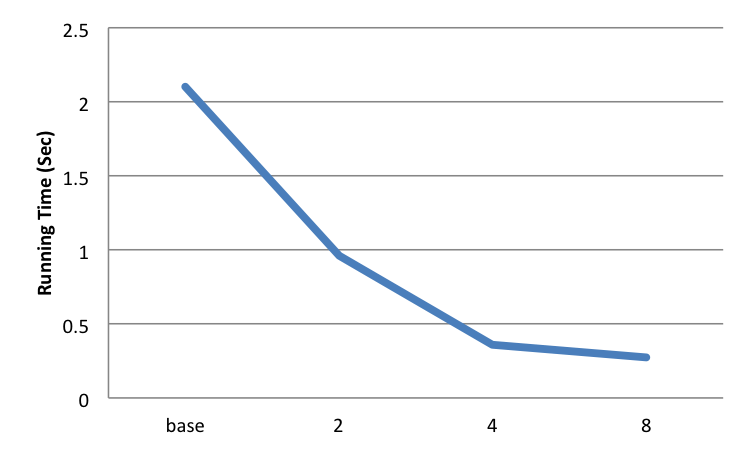
\includegraphics[width=200pt]{/Users/chayong/Documents/project2/figs/seq_runtime.png}}
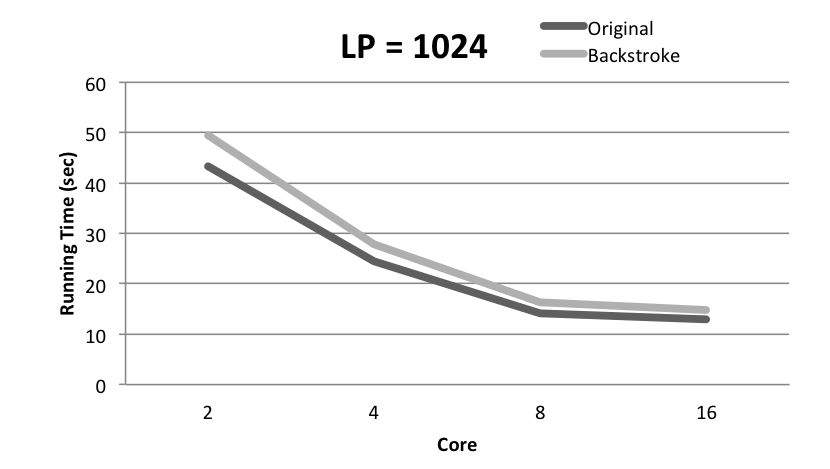
\includegraphics[width=3.0in]{figs/p_runtime_1024.png}
\end{minipage}
&
\begin{minipage}{200pt}
%\frame{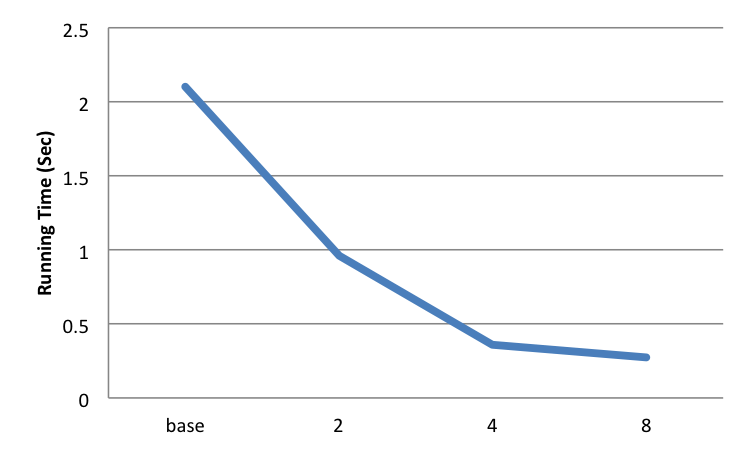
\includegraphics[width=250pt]{/Users/chayong/Documents/project2/figs/seq_runtime.png}}
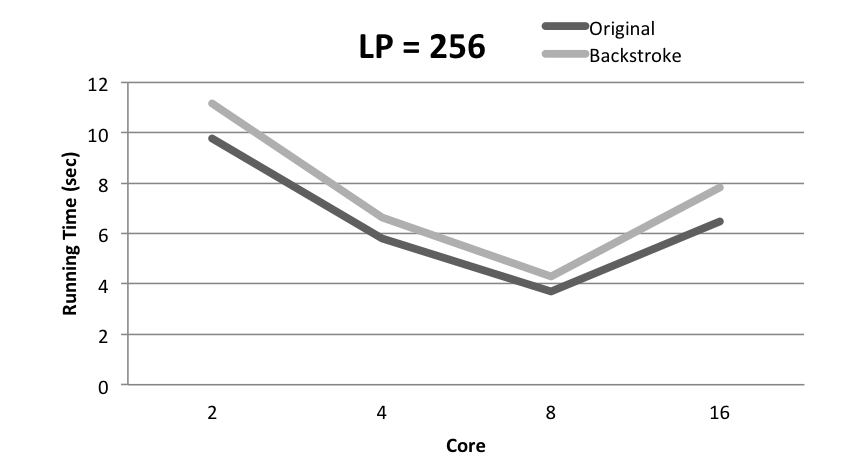
\includegraphics[width=3.0in]{figs/p_runtime_256.png}

\end{minipage}
\end{tabular}
\caption{Simulation Performance Using Different Numbers of Processors}
\label{fig:p_runtime}
\end{figure}



As we can see from the figure \ref{fig:p_runtime}, the simulation execution time decreased as we increased the number of cores.
In the case of benchmark with 256 LPs, we experienced a more overhead on using 16 cores, which results in decreasing the simulation performance. 